\documentclass[twocolumn,11pts]{IEEEtran}
% opciones para utilizar el español

\makeatletter
\adddialect\l@SPANISH\l@spanish
\makeatother
\usepackage[spanish,es-lcroman,es-tabla,es-nosectiondot]{babel}
\decimalpoint% cambia las comas a puntos
\usepackage[utf8]{inputenc}
\usepackage{csquotes}

\usepackage{textcomp}%incluye el comando \texttildelow

% *** CAPTION ***
\usepackage[font=footnotesize,labelfont=bf,labelsep=period]{caption}

% *** CITATION PACKAGES ***
% Cargar el paquete cite hará que las citas sean ordenadas y comprimidas
% automáticamente. E.g., [1], [9], [2], [7], [5], [6] sin utilizar cite.sty
% se convertirán en [1], [2], [5]--[7], [9]. 
\usepackage{cite}


% *** CITATION PACKAGES ***
%
\usepackage{cite}

\usepackage{filecontents}
\begin{filecontents}{refs.bib}
% note el uso de las llaves {} para escapar la instrucción \LaTeX dentro del título del artículo
@article{ourpaper,
  author = {Haque, Sk. Mohammadul and Chatterjee, Avishek and Govindu, Venu Madhav},
  title = {High Quality Photometric Reconstruction from a Depth Camera},
  booktitle = {2014 IEEE Conference on Computer Vision and Pattern Recognition (CVPR)},
  year = {2014},
  organization = {IEEE},
  url = {http://www.ee.iisc.ernet.in/labs/cvl/papers/photometric_CVPR2014_paper.pdf}
}

@article{dos,
author={Qing Zhang and Mao Ye and Ruigang Yang and Matsushita, Y. and Wilburn, B. and Huimin Yu},
booktitle={Computer Vision and Pattern Recognition (CVPR), 2012 IEEE Conference on},
title={Edge-preserving photometric stereo via depth fusion},
year={2012},
month={June},
pages={2472-2479},
keywords={edge detection;image fusion;iterative methods;optimisation;stereo image processing;active stereo;depth fusion;edge-preserving photometric stereo;ill-conditioned pixels;image-based heuristics;iterative optimization scheme;nonlinear cost function;sensor fusion scheme;shadow area detection;Cameras;Image reconstruction;Light sources;Lighting;Optimization;Sensor fusion;Stereo vision},
doi={10.1109/CVPR.2012.6247962},
ISSN={1063-6919},}
@book{libro,
  author = {Richard {S}zeliski},
  title = {Computer {V}ision:{A}lgorithms and {A}pplications},
  year = {2010},
  url = {http://szeliski.org/Book/}
}

@incollection{Woodham,
 author = {Woodham, Robert J.},
 chapter = {Photometric Method for Determining Surface Orientation from Multiple Images},
 title = {Shape from Shading},
 editor = {Horn, Berthold K. P. and Brooks, Michael J.},
 year = {1989},
 isbn = {0-262-08183-0},
 pages = {513--531},
 numpages = {19},
 url = {http://dl.acm.org/citation.cfm?id=93871.93888},
 acmid = {93888},
 publisher = {MIT Press},
 address = {Cambridge, MA, USA},
} 

@article{Nehab,
 author = {Nehab, Diego and Rusinkiewicz, Szymon and Davis, James and Ramamoorthi, Ravi},
 title = {Efficiently Combining Positions and Normals for Precise 3D Geometry},
 journal = {ACM Trans. Graph.},
 issue_date = {July 2005},
 volume = {24},
 number = {3},
 month = jul,
 year = {2005},
 issn = {0730-0301},
 pages = {536--543},
 numpages = {8},
 url = {http://doi.acm.org/10.1145/1073204.1073226},
 doi = {10.1145/1073204.1073226},
 acmid = {1073226},
 publisher = {ACM},
 address = {New York, NY, USA},
}
@inproceedings{Han,
    AUTHOR = {Yudeog Han and Joon-Young Lee and In So Kweon},
    TITLE = {High Quality Shape from a Single RGB-D Image under Uncalibrated Natural Illumination},
    BOOKTITLE = {Proceedings of IEEE International Conference on Computer Vision (ICCV)},
    YEAR = {2013}
}

@incollection{Horn,
 author = {Horn, Berthold K. P.},
 chapter = {Obtaining Shape from Shading Information},
 title = {Shape from Shading},
 editor = {Horn, Berthold K. P. and Brooks, Michael J.},
 year = {1989},
 isbn = {0-262-08183-0},
 pages = {123--171},
 numpages = {49},
 url = {http://dl.acm.org/citation.cfm?id=93871.93877},
 acmid = {93877},
 publisher = {MIT Press},
 address = {Cambridge, MA, USA},
} 

@MISC{elotro,
    author = {Grant Schindler},
    title = {Photometric Stereo via Computer Screen Lighting for Real-time Surface Reconstruction},
    year = {}
}

@link{repo,
title={Uncalibrated-Photometric-Stereo},
author={Kai Wolf},
url={https://github.com/NewProggie/Uncalibrated-Photometric-Stereo},
}
\end{filecontents}

% *** GRAPHICS RELATED PACKAGES ***
%
\usepackage{graphicx}
% las rutas donde están los archivos
% \graphicspath{{../pdf/}{../jpeg/}}
% y las extensiones que se usarán, así no se declaran al incluir la imagen
% \DeclareGraphicsExtensions{.pdf,.jpeg,.png}


% *** MATH PACKAGES ***
% Provee varios comandos para trabajar con matemáticas. Si se utiliza, cargelo
% con la opción cmex10 para asegurar que solamente fuentes tipo 1 (type 1 fonts)
% sean utilizadas para todos los tamaños. Sin esta opción, es posible que
% algunos símbolos sean colocados en bitmaps, particularmente en notas al pie
% de página.
\usepackage[cmex10]{amsmath}
% Adicionalmente el paquete establece \interdisplaylinepenalty a 10000
% lo que previene que las páginas terminen dentro de ecuaciones múltiples.
% Utilice 
\interdisplaylinepenalty=2500
% para restablecer el comportamiento normal de IEEEtran.cls


% *** SPECIALIZED LIST PACKAGES ***
% Los paquetes para escribir algoritmos y pseudocódigo
\usepackage{algorithm}
\usepackage{algpseudocode}
\makeatletter
\renewcommand{\ALG@name}{Algoritmo}% Algorithm -> Algoritmo
\makeatother
\captionsetup[algorithm]{font=footnotesize,labelsep=period}

% Paquetes para escribir código
\usepackage{listings}
\usepackage{tikz}
\lstset{
  language=[LaTeX]TeX,
  breaklines=true,
  basicstyle=\tt\scriptsize,
  keywordstyle=\color{blue},
  identifierstyle=\color{magenta},
  commentstyle=\color{green!40!black},
  % frame 
  frame=tb,
  captionpos=t,
  xleftmargin=1em,
  numbersep=0.3em,
  numbers=left,
  framexleftmargin=1.1em,
  framexrightmargin=0pt,
  % additional letters for accents in spanish
  literate=%
    {á}{{\'{a}}}1
    {é}{{\'{e}}}1
    {í}{{\'{i}}}1
    {ó}{{\'{o}}}1
    {ú}{{\'{u}}}1
    {ñ}{{\~{n}}}1
    {Ñ}{{\~{N}}}1
}

\renewcommand{\lstlistingname}{Código}% Listing -> Código
\DeclareCaptionFormat{listing}{\rule{\dimexpr\linewidth\relax}{0.4pt}\par\vskip1pt#1#2#3}
\captionsetup[lstlisting]{format=listing,singlelinecheck=false, margin=0pt,position=bottom}


% *** ALIGNMENT PACKAGES ***
% Este paquete extiende las funcionalidades de las tablas (tabular)
\usepackage{tabularx}
% Este paquete repara y mejora los paquetes estándar: array y tabular.
%\usepackage{array}


%\usepackage{mdwmath}
%\usepackage{mdwtab}
% Also highly recommended is Mark Wooding's extremely powerful MDW tools,
% especially mdwmath.sty and mdwtab.sty which are used to format equations
% and tables, respectively. The MDWtools set is already installed on most
% LaTeX systems. The lastest version and documentation is available at:
% http://www.ctan.org/tex-archive/macros/latex/contrib/mdwtools/


% IEEEtran contains the IEEEeqnarray family of commands that can be used to
% generate multiline equations as well as matrices, tables, etc., of high
% quality.


%\usepackage{eqparbox}
% Also of notable interest is Scott Pakin's eqparbox package for creating
% (automatically sized) equal width boxes - aka "natural width parboxes".
% Available at:
% http://www.ctan.org/tex-archive/macros/latex/contrib/eqparbox/


% *** SUBFIGURE PACKAGES ***
% Permite utilizar las figuras y subfiguras utilizando el comando \float
\usepackage[font=footnotesize,caption=false,labelformat=simple]{subfig}
% el siguiente código permite utilizar paréntesis de manera automática
% al citar subfiguras, e.g., Fig. 1(a)
\renewcommand\thesubfigure{(\alph{subfigure})}
\renewcommand\thesubtable{(\alph{subtable})}
\newcommand{\subfigureautorefname}{\figureautorefname}


% *** FLOAT PACKAGES ***
%
%\usepackage{fixltx2e}
% fixltx2e, the successor to the earlier fix2col.sty, was written by
% Frank Mittelbach and David Carlisle. This package corrects a few problems
% in the LaTeX2e kernel, the most notable of which is that in current
% LaTeX2e releases, the ordering of single and double column floats is not
% guaranteed to be preserved. Thus, an unpatched LaTeX2e can allow a
% single column figure to be placed prior to an earlier double column
% figure. The latest version and documentation can be found at:
% http://www.ctan.org/tex-archive/macros/latex/base/

%\usepackage{stfloats}
% stfloats.sty was written by Sigitas Tolusis. This package gives LaTeX2e
% the ability to do double column floats at the bottom of the page as well
% as the top. (e.g., "\begin{figure*}[!b]" is not normally possible in
% LaTeX2e). It also provides a command:
%\fnbelowfloat
% to enable the placement of footnotes below bottom floats (the standard
% LaTeX2e kernel puts them above bottom floats). This is an invasive package
% which rewrites many portions of the LaTeX2e float routines. It may not work
% with other packages that modify the LaTeX2e float routines. The latest
% version and documentation can be obtained at:
% http://www.ctan.org/tex-archive/macros/latex/contrib/sttools/
% Documentation is contained in the stfloats.sty comments as well as in the
% presfull.pdf file. Do not use the stfloats baselinefloat ability as IEEE
% does not allow \baselineskip to stretch. Authors submitting work to the
% IEEE should note that IEEE rarely uses double column equations and
% that authors should try to avoid such use. Do not be tempted to use the
% cuted.sty or midfloat.sty packages (also by Sigitas Tolusis) as IEEE does
% not format its papers in such ways.

%\ifCLASSOPTIONcaptionsoff
%  \usepackage[nomarkers]{endfloat}
% \let\MYoriglatexcaption\caption
% \renewcommand{\caption}[2][\relax]{\MYoriglatexcaption[#2]{#2}}
%\fi
% endfloat.sty was written by James Darrell McCauley and Jeff Goldberg.
% This package may be useful when used in conjunction with IEEEtran.cls'
% captionsoff option. Some IEEE journals/societies require that submissions
% have lists of figures/tables at the end of the paper and that
% figures/tables without any captions are placed on a page by themselves at
% the end of the document. If needed, the draftcls IEEEtran class option or
% \CLASSINPUTbaselinestretch interface can be used to increase the line
% spacing as well. Be sure and use the nomarkers option of endfloat to
% prevent endfloat from "marking" where the figures would have been placed
% in the text. The two hack lines of code above are a slight modification of
% that suggested by in the endfloat docs (section 8.3.1) to ensure that
% the full captions always appear in the list of figures/tables - even if
% the user used the short optional argument of \caption[]{}.
% IEEE papers do not typically make use of \caption[]'s optional argument,
% so this should not be an issue. A similar trick can be used to disable
% captions of packages such as subfig.sty that lack options to turn off
% the subcaptions:
% For subfig.sty:
% \let\MYorigsubfloat\subfloat
% \renewcommand{\subfloat}[2][\relax]{\MYorigsubfloat[]{#2}}
% For subfigure.sty:
% \let\MYorigsubfigure\subfigure
% \renewcommand{\subfigure}[2][\relax]{\MYorigsubfigure[]{#2}}
% However, the above trick will not work if both optional arguments of
% the \subfloat/subfig command are used. Furthermore, there needs to be a
% description of each subfigure *somewhere* and endfloat does not add
% subfigure captions to its list of figures. Thus, the best approach is to
% avoid the use of subfigure captions (many IEEE journals avoid them anyway)
% and instead reference/explain all the subfigures within the main caption.
% The latest version of endfloat.sty and its documentation can obtained at:
% http://www.ctan.org/tex-archive/macros/latex/contrib/endfloat/
%
% The IEEEtran \ifCLASSOPTIONcaptionsoff conditional can also be used
% later in the document, say, to conditionally put the References on a 
% page by themselves.


% *** PDF, URL AND HYPERLINK PACKAGES ***
% Provee una forma de manejar y romper URLs. Se utiliza como \url{mi_url_aca}.
\usepackage{url}
\urlstyle{tt}
% *** Do not adjust lengths that control margins, column widths, etc. ***
% *** Do not use packages that alter fonts (such as pslatex).         ***
% There should be no need to do such things with IEEEtran.cls V1.6 and later.
% (Unless specifically asked to do so by the journal or conference you plan
% to submit to, of course. )

% this should be the latest package to load (unless you find an exception or 
% clash between packages)
\usepackage{hyperref}
\hypersetup{
  colorlinks=false,       % false: boxed links; true: colored links
  pdfborder={0 0 0}       % remove ugly border from links
}

% *** Definiciones ***
\usepackage{xspace}
\makeatletter
\DeclareRobustCommand\onedot{\futurelet\@let@token\@onedot}
\def\@onedot{\ifx\@let@token.\else.\null\fi\xspace}

\def\eg{\emph{e.g}\onedot} \def\Eg{\emph{E.g}\onedot}
\def\ie{\emph{i.e}\onedot} \def\Ie{\emph{I.e}\onedot}
\def\cf{\emph{cf}\onedot} \def\Cf{\emph{Cf}\onedot}
\def\etc{\emph{etc}\onedot} \def\vs{\emph{vs}\onedot}
\def\wrt{w.r.t\onedot} \def\dof{d.o.f\onedot}
\def\etal{\emph{et al}\onedot}
\def\adhoc{\emph{ad hoc}\xspace}
\makeatother


% correct bad hyphenation here
\hyphenation{op-tical net-works semi-conduc-tor}
\usepackage{enumerate}

\begin{document}
%
% paper title
% can use linebreaks \\ within to get better formatting as desired
\title{Informe proyecto final.}
%

\author{Daniel Méndez~\IEEEmembership{Miembro~IEEE,} Camila Sanhueza~\IEEEmembership{Miembro~IEEE}% 

\thanks{mail: daniel.mendezf@mail.udp.cl}%
\thanks{mail: camila.sanhueza@mail.udp.cl}%
% <-this % stops a space
}
% note the % following \thanks
% these prevent an unwanted space from occurring between the last author name
% and the end of the author line. i.e., if you had this:
% 
% \author{....lastname \thanks{...} \thanks{...} }
%                     ^------------^------------^----Do not want these spaces!
%
% a space would be appended to the last name and could cause every name on that
% line to be shifted left slightly. This is one of those "LaTeX things". For
% instance, "\textbf{A} \textbf{B}" will typeset as "A B" not "AB". To get
% "AB" then you have to do: "\textbf{A}\textbf{B}"
% \thanks is no different in this regard, so shield the last } of each \thanks
% that ends a line with a % and do not let a space in before the next \thanks.
% Spaces after \IEEEmembership other than the last one are OK (and needed) as
% you are supposed to have spaces between the names. For what it is worth,
% this is a minor point as most people would not even notice if the said evil
% space somehow managed to creep in.


% The paper headers
\markboth{Visión por computador}%
{Reporte}%<- this part will appear only with the twoside option in the documentclass
% The only time the second header will appear is for the odd numbered pages
% after the title page when using the twoside option.

% make the title area
\maketitle
\begin{abstract}
Basados en el paper de Hake~\cite{ourpaper}, en este informe mostramos los resultados que obtuvimos al intentar hacer la reconstrucción 3D de un objeto, siguiendo lo expuesto por Hake. 

Para comenzar, introducimos explicando las dificultades que se nos presentaron durante el proceso. También definimos las diferencias del resultado final con lo que propusimos al comenzar el desarrollo del proyecto. Hemos de explicar también, el diseño y la implementación del código generado y utilizado. 

Se muestran también en detalle los resultados obtenidos y un análisis de éstos.
\end{abstract}


\section{Introducción}
La reconstrucción en 3D de un objeto, es un área que tiene muchos, y muy variados, acercamientos. Desde 1980 con la introducción de métodos fotométricos, o a través de la técnica llamada \textit{shape-from-shading}, se ha intentado construir en realidad aumentada los objetos en el computador.

Con la puesta en el mercado de la Kinect, se presentó una nueva forma de lograr el tan anhelado objetivo. Es así como nuevas mentes encontraron formas distintas de hacer una construcción en tres dimensiones.

Para éste proyecto, partimos basándonos en el paper de Hake~\cite{ourpaper}, el cual plantea el uso del receptor infrarrojo para captar las diferentes imágenes del objeto. Además sugiere usar una fuente externa de luz infrarroja, para obtener mejores resultados de resolución a la hora de reconstruir. Los problemas al querer seguir este método, se presentaron a la hora de obtener las normales para hacer el mapa de profundidad, dado que la documentación de Hake es escasa al ser un método propuesto por él. 

Para resolver este problema, combinamos el acercamiento de Hake con el de Schindler~\cite{elotro}. Usamos fotometría no calibrada para hacer el calculo de las normales a partir de 4 fotos tomadas con la Kinect y con una fuente externa de luz infrarroja. Luego, para el armar el mapa de profundidad, utilizamos el método de Gauss-Seidel con relajación.

Finalmente, las pruebas son generadas haciendo una modificación del código de Kai Wolf~\cite{repo}, para adaptarlo a nuestras condiciones de trabajo, es decir, utilizar la Kinect como cámara y la fuente externa de luz infrarroja.
 
\section{Diseño e implementación }
Para lograr el objetivo de realizar reconstrucciones $3D$, utilizamos el código de Kai Wolf, que nos brindaba la fotometría no calibrada~\cite{repo}. A éste trabajo le realizamos una serie de modificaciones y agregamos el código que nos permite utilizar la Kinect como cámara capturadora. Para poder realizar las reconstrucciones en $3D$ utilizamos una luz infrarroja, que no entregó resultados favorables. Cambiamos entonces a una halógena con filtro dicroico, filtro que aporta un componente infrarrojo suficiente para captarlo conla Kinect, pero no tan fuerte como la luz infrarroja.
\subsection{Código que permite la utilización de la Kinect}
\begin{itemize}
\item Diseño: Al momento de analizar el uso de la Kinect, se nos presentaron diferentes librerías (\texttt{OpenNi, Freenect, etc}) que nos brindaban herramientas para el desarrollo. Al momento de realizar pruebas con las librerías mencionadas, ninguna resultó de la forma deseada. Lo que nos obligó a recurrir a otros medios, llegando finalmente a utilizar \texttt{Openframenworks}.

\item Implementación: para poder utilizar la Kinect como sensor de profundidad y de intensidades. Usamos las herramientas de \texttt{Openframenworks}, específicamente \texttt{ofxKinect}. Este código nos permite obtener y almacenar las imágenes de intensidad y mapas de profundidad de las pruebas. Esto se realiza al presionar la tecla ``S'', con la que podemos almacenar las intensidades del frame que en ese instante esta siendo visto por la Kinect. Al presionar ``D'', almacenamos los mapas de profundidad. El funcionamiento de esta libreria consiste en que es necesario determinar las variables esenciales a utilizar en el archivo \texttt{ofApp.h}, el cual crea una clase. En el archivo \texttt{ofApp.cpp} se encuentra las siguientes funciones: setup, update y draw, que siempre se ejecutan el orden mencionado, luego se continua realizando ciclos entre update y draw. 
La función \texttt{setup} configura las opciones necesarias para iniciar la Kinect, \texttt{update} como su nombre lo indica, renueva la información entregada por la Kinect y finalmente \texttt{draw}, dibuja la información necesaria en la pantalla. Además incluye la función \texttt{pressKey}, que permite realizar acciones al presionar diferentes teclas.
\end{itemize}


\subsection{Código de la fotometría no calibrada}
\subsubsection{Función \texttt{exportMesh}}
\begin{itemize}
\item Diseño: esta función nos permite transformar la información de las matrices de profundidad y de normales, en una representación $3d$. Para poder visualizar las reconstrucciones realizadas utilizamos la herramienta \texttt{meshlab}.
\begin{lstlisting}[float,language=C++,caption={Prototipo función \texttt{exportMesh}.},label=cod:c0]
void exportMesh(cv::Mat Depth, cv::Mat Normals, cv::Mat texture);
\end{lstlisting}
\item Implementación: es función las variables \texttt{ofstream}, en donde esta crea un archivo con extensión \texttt{.obj} en donde los datos son ingresados escribiendo en el mismo archivo los valores necesarios de estas matrices.
\end{itemize}
\subsubsection{Función \texttt{imageMask}}
\begin{itemize}
\item Diseño: esta función consiste en eliminar todo el fondo de la imagen, transformándolo a color negro. Donde se encuentra el objeto de prueba, se deja la silueta del objeto, rellenándolo con color blanco.
\begin{lstlisting}[float,language=C++,caption={Prototipo función \texttt{imageMask}.},label=cod:c1]
Mat imageMask(vector<Mat> camImages, int numPics, Mat ambient);
\end{lstlisting}
\item Implementación: en el código~\ref{cod:c1} se puede observar el prototipo de esta función. El parámetro \texttt{camUmagenes}, es un vector que posee las imágenes de las distintas iluminaciones, \texttt{numPics} son las cantidad de imágenes que posee este arreglo y finalmente el \texttt{ambiente} es una imagen más oscura para obtener el fondo. Para obtener la mascara se sumaron todas las imágenes y se les restó el ambiente. Para no obtener valores fuera del rango de escala de grises se realiza un threshold.


\end{itemize}
\subsubsection{Función \texttt{computeNormals}}
\begin{itemize}
\item Diseño: esta función consiste en calcular la normal para cada pixel de las imágenes, y asignarle  a la matriz resultante un valor que es representado con diferentes colores. Como no se podía controlar o calibrar las fuentes de iluminación, fue necesario utilizar un método de fotometría estero no calibrada. 
\begin{lstlisting}[float,language=C++,caption={Prototipo función \texttt{computeNormals}.},label=cod:c2]
Mat computeNormals(vector<Mat> camImages,Mat Mask =Mat());
\end{lstlisting}
\item Implementación: al igual que en la función anterior se le entrega el arreglo de imágenes, más la mascara calculada anteriormente. Inicialmente esta función crea una matriz que almacene la información de intensidad de las fotos y en las diferentes columnas de esta se representan imágenes con diferentes iluminaciones. Posterior a crear esta matriz se le realiza una descomposición de valores singulares para obtener los valores propios y así poder obtener la información en una matriz de tres canales (RGB).
\end{itemize}
\subsubsection{Función \texttt{cvtFloatToGrayscale}}
\begin{itemize}
\item Diseño: esta función, tal como su nombre lo dice, transforma una matriz de valores flotantes a un matriz en escala de grises.

\begin{lstlisting}[float,language=C++,caption={Prototipo función \texttt{cvtFloatToGrayscale}.},label=cod:c3]
Mat cvtFloatToGrayscale(cv::Mat F, int limit = 255);
\end{lstlisting}

\item Implementación: en el código~\ref{cod:c3} se ingresa una matriz para que sea transformada a una escala de grises, principalmente a valores que no sobrepasen el 255.

\end{itemize}
\subsubsection{Función \texttt{localHeightfield}}
\begin{itemize}
\item Diseño: esta función nos permite, a través del calculo de de normales, realizar una estimación de las profundidades de la imagen. Se utiliza el método de Gauss-Seidel con relajación, de esta manera se calcula la profundidad mediante un método iterativo, actualizando el valor de cada pixel en relación a su vecindario. De esta forma se utilizan los valores de las normales y el mapa de profundidad, que comienza siendo plano, va aumentando la profundidad a medida que avanzan las iteraciones.
\begin{lstlisting}[float,language=C++,caption={Prototipo función \texttt{localHeigthfield}.},label=cod:c4]
Mat localHeightfield(cv::Mat Normals);
\end{lstlisting}
\item Implementación: para estimar las profundidades se realizaron iteraciones sobre una serie de pirámides de la matriz de las normales. En éstas iteraciones se calcula la profundidad de un píxel mediante el análisis de su vecindario. Después de la estimación de esta matriz de profundidad, buscamos los valores máximos y mínimos para que nuestra profundidad no supere estos valores.
\end{itemize}
\subsubsection{Función \texttt{E\_d}}
\begin{itemize}
\item Diseño: como menciona Hake~\cite{ourpaper} en su paper, es necesario realizar diferentes funciones de costos, una de estas es calcular el costo para las normales. Este se rige por
\begin{equation} \label{eq:1}
E_d(\hat{Z})= \sum_{p} w_p ||u_p||^{2}(Z_{p}-\hat{Z_p})^{2}
\end{equation}%
donde $u_p=[ {\frac{-x}{f}}  {\frac{-y}{f}}  1]^{T}$, $w_p$ representa los valores propios de $\sum_q N_{q}N_{q}^{T}$ y donde $Z$ representa las profundidades para los distintos valores de los pixeles.
\item Implementación: para este se implementó la ecuación~\ref{eq:1}, para cada valor de las distintas profundidades, ya que se ingresan las profundidades estimadas y las profundidades calculadas con la Kinect.
\end{itemize}
\subsubsection{Función \texttt{E\_n}}
\begin{itemize}
\item Diseño: para el costo de las normales, se utilizo la siguiente formula
\begin{equation} \label{eq:2}
E_n(\hat{Z})= \sum_{p} (N_p T_x)^2 + (N_p T_y)^2,
\end{equation}
donde $T_x$ y $T_y$, representan las derivadas parciales a sus respectivos ejes en $Z$ y donde $N_p$  es el valor de la normal para el píxel $p$.
\item Implementación: para implementar esta función se utilizo la ecuación~\ref{eq:2}, realizando la sumatoria de todos los pixeles con los valores antes mencionados.
\end{itemize}
\subsubsection{Función \texttt{E\_s}}
\begin{itemize}
\item Diseño: del mismo modo que las funciones anteriores este se rige por $\bigtriangledown^2(\hat{Z})$, en cual es el operador Laplaciano para coordenadas cartesianas.
\item Implementación:para realizar esto es necesario realizar las deribadas de $Z$ con respecto a los ejes $x$ e $y$. Para esto se utilizo la función de \texttt{sobel} implementada por \texttt{openCV}, se realizo dos veces cada derivada a los diferentes ejes y luego estas se sumaron.
\end{itemize}
\subsubsection{Función \texttt{main}}
en esta función se utilizan todas las funciones mencionadas anteriormente, el orden de esto generar las mascaras de las imágenes, se elimina el fondo de las imágenes con la mascara ,se calculan las normales, se calculan las profundidades y finalmente se realiza el mesh.


\section{Experimentos}
Como mencionamos anteriormente, nos basamos en el código de Kai Wolf~\cite{repo} para obtener las normales y el mapa de profundidad, pero le aplicamos algunos cambios que se reflejaron en reconstrucciones de mejor calidad. 

Siguiendo la idea de Hake, decidimos aplicarle un filtro Gaussiano a las imágenes obtenidas con la Kinect, para eliminar ruido y lograr mayor suavidad en las reconstrucciones. Una vez obtenidas las fotos, hicimos el procesamiento de la máscara (Ver figura~\ref{mascaras}), y le aplicamos un \texttt{bitwise\_and} a las imágenes con ésta. Éste proceso Wolf no lo hacía, solo aplicaba la máscara a las normales. Hacer este cambio nos permitió eliminar mejor el fondo y trabajar solo con los datos que nos interesaban. En la figura~\ref{comparacion}, se puede ver una comparación de ambos métodos. Usando las imágenes de ejemplo proporcionadas por Kai Wolf, hicimos la reconstrucción usando ambos algoritmos. 

\begin{figure}[t]
\begin{center}
	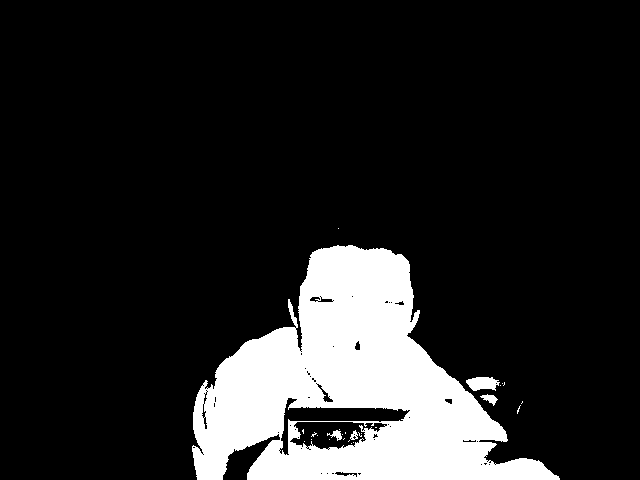
\includegraphics[width= 4cm]{Mascaracrepu}
	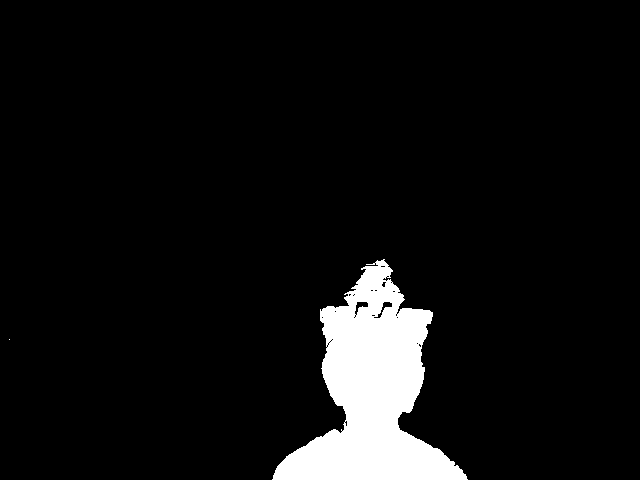
\includegraphics[width= 4cm]{Mascaramona}
	
\includegraphics[width= 4cm]{Mascaraniple}
		\caption{Mascaras auto-generadas para eliminar el fondo.}
		\label{mascaras}
\end{center}
\end{figure}

\begin{figure*}[bt]%prefer bottom (b) and then top (t)
\centering
\subfloat[Reconstrucción de Wolf.]{%<- this stops spurious white spaces
  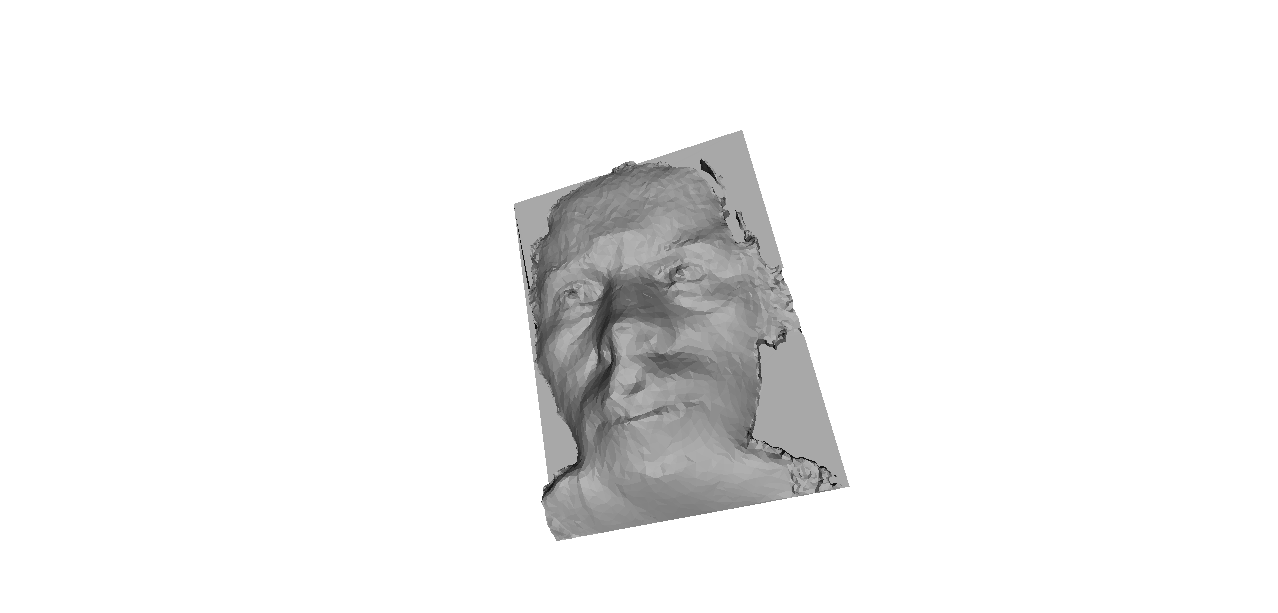
\includegraphics[width= 8cm]{3dwolfwolf00}
  \label{asd}
}%
\subfloat[Reconstrucción nuestra.]{%
  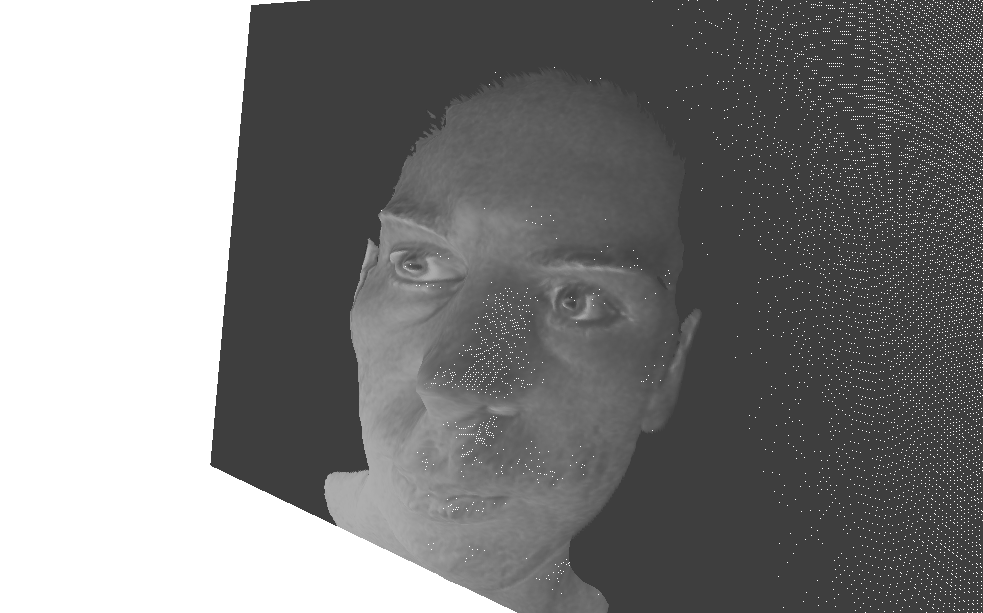
\includegraphics[width= 6cm]{3dwolfnuestro01}
  \label{qwe}
}
\caption{Comparación del algoritmo de Wolf y el nuestro para la reconstrucción.}
\label{comparacion}
\end{figure*}

Luego de obtener las imágenes y pre procesarlas, encontramos las normales y el mapa de profundidad. Para calcular las normales, se necesita la suma de las 4 fotos, menos la mascara. A partir de esta imagen se construyen las normales. El mapa de profundidad, se obtiene con la información de la máscara y de la textura de la imagen, para la cual se usa una de las 4 previamente capturadas. La figura~\ref{normal} y la figura~\ref{profundidad}, muestran las normales y el mapa de profundidad respectivamente.

\begin{figure}[t]
\begin{center}
	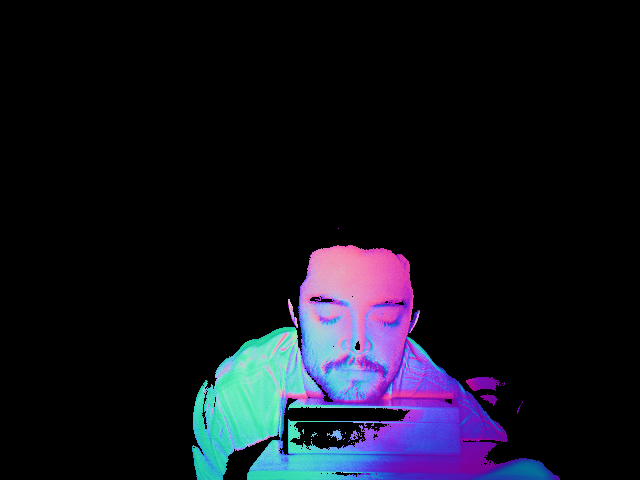
\includegraphics[width= 4cm]{Normalcrepu}
	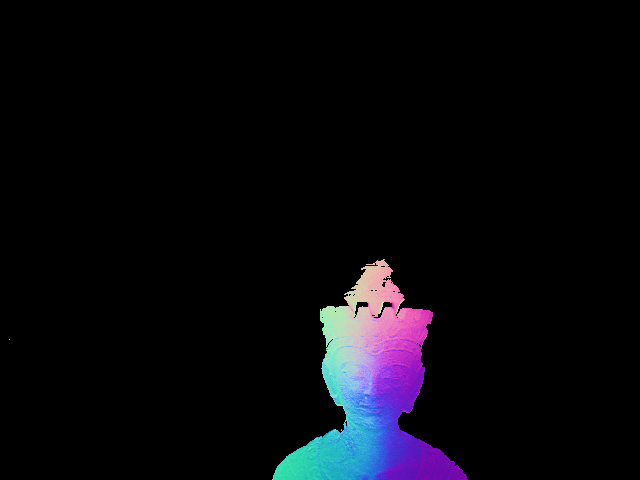
\includegraphics[width= 4cm]{Normalmona}
	
\includegraphics[width= 4cm]{Normalniple}
		\caption{Imágenes que representan las normales.}
		\label{normal}
\end{center}
\end{figure}

\begin{figure}[t]
\begin{center}
	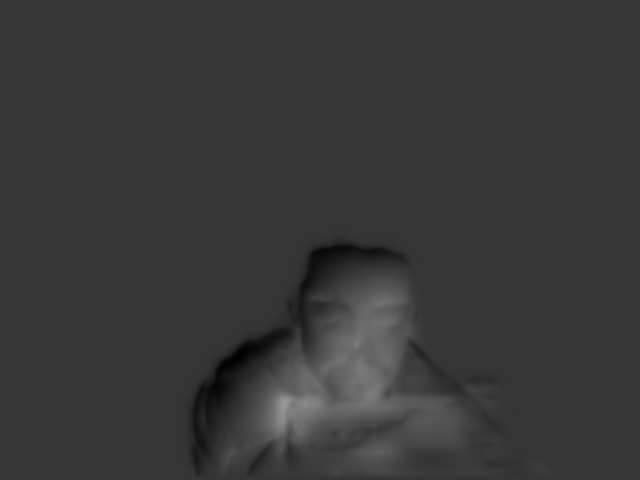
\includegraphics[width= 4cm]{Profundidadcrepu}
	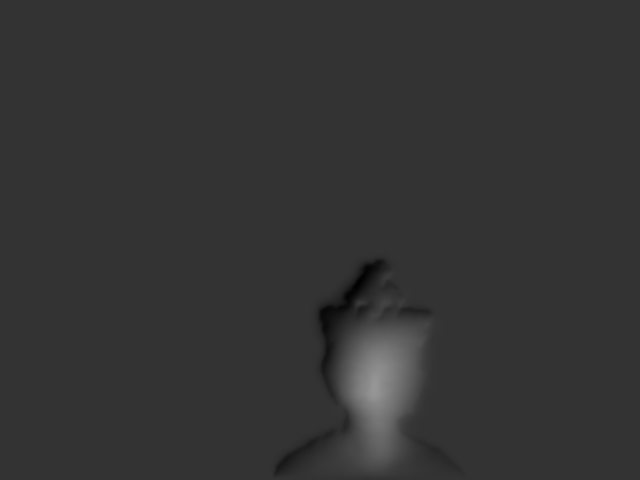
\includegraphics[width= 4cm]{Profundidadmona}
	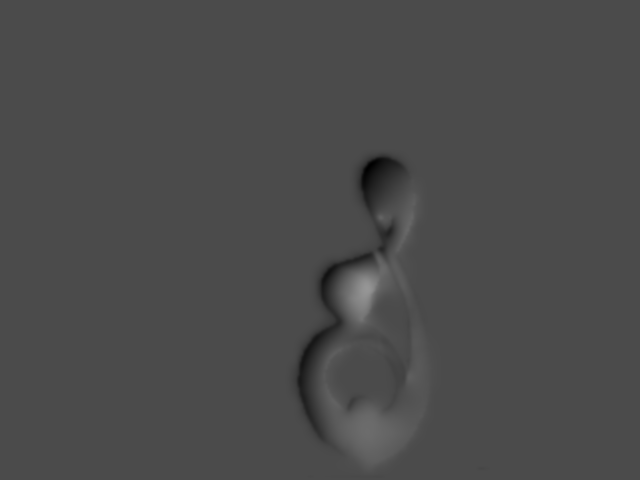
\includegraphics[width= 4cm]{Profundidadniple}
		\caption{Ejemplos de mapas de profundidad.}
		\label{profundidad}
\end{center}
\end{figure}

Durante el desarrollo del proyecto, tuvimos varios problemas para armar el set-up de Kai Wolf. Esto debido a la dificultad para controlar el ambiente. Uno de los problemas que tuvimos fue la luz infrarroja. La primera que teníamos era muy grande y de luminosidad muy fuerte. Esto producía que el objeto se viera en extremo iluminado y que por ende su mapa de profundidad no sea adecuado. La figura~\ref{crepu}, muestra un resultado fallido.

\begin{figure}[t]
\begin{center}
	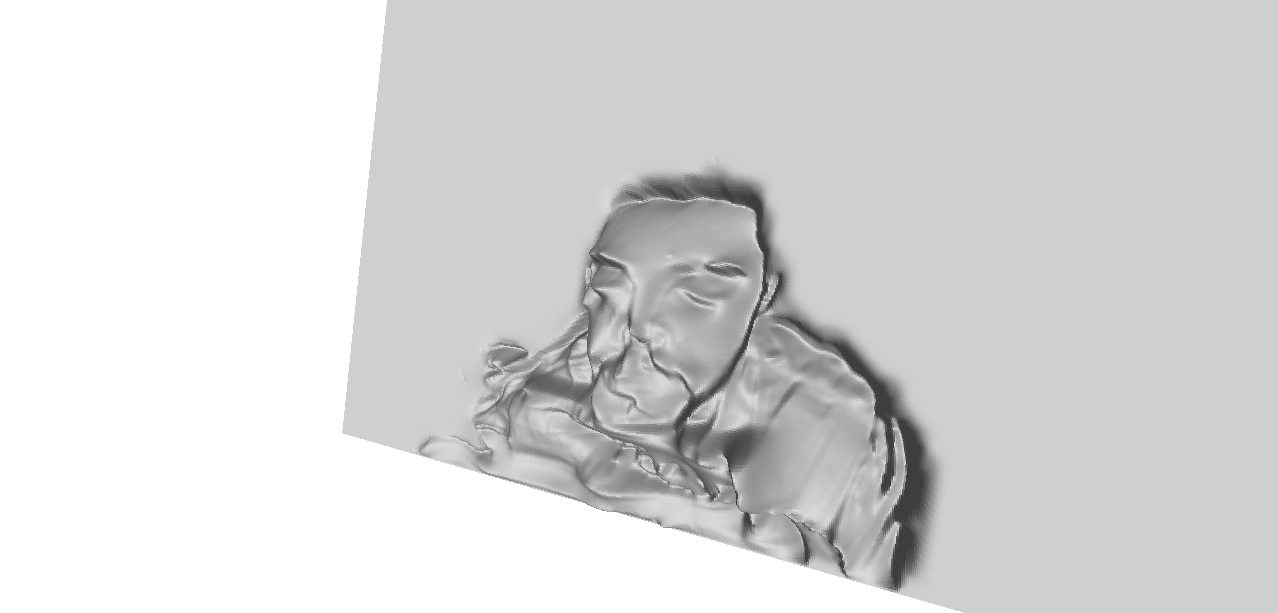
\includegraphics[width= 5cm]{3dcrepu00}
		\caption{Reconstrucción 3D fallida.}
		\label{crepu}
\end{center}
\end{figure}

A pesar de todo esto, logramos obtener reconstrucciones que definimos como exitosas. Pudimos conseguir una ampolleta más pequeña con componente infrarrojo suficiente para poder captarla con la Kinect. Además, encontramos objetos de prueba que cumplían con las características requeridas por la fotomometría estereo, es decir, eran lambertianos. La figura~\ref{mona} y~\ref{niple}, muestran estos resultados.

\begin{figure}[t]
\begin{center}
	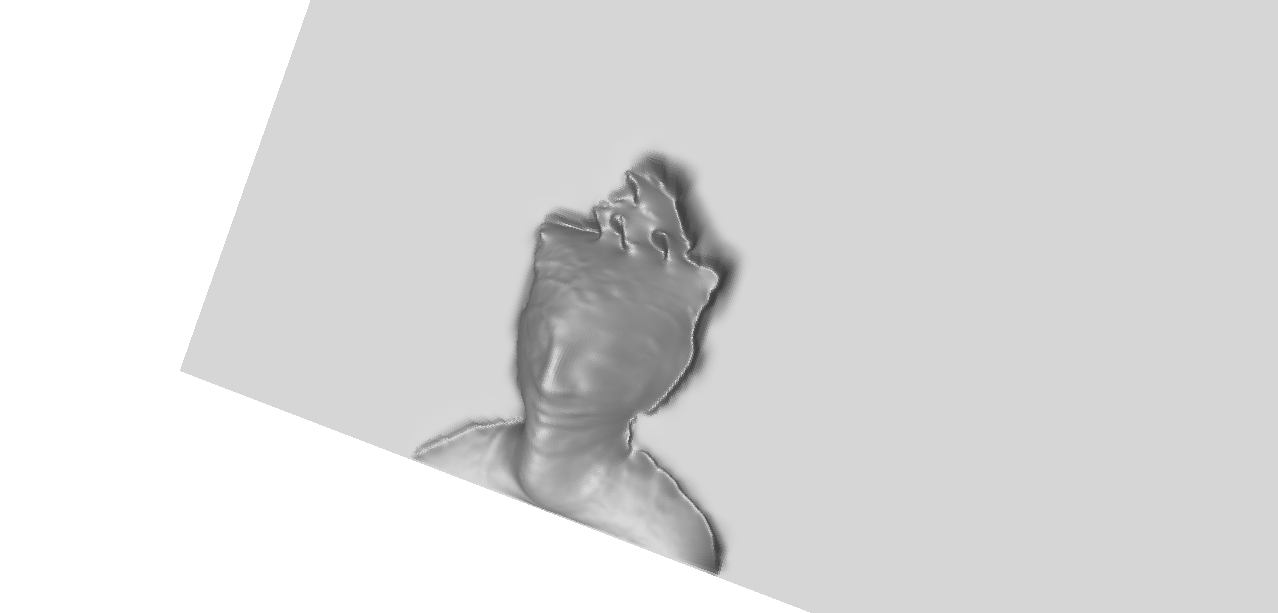
\includegraphics[width= 5cm]{3dmona01}
		\caption{Reconstrucción 3D de una figura de buda.}
		\label{mona}
\end{center}
\end{figure}

\begin{figure}[t]
\begin{center}
	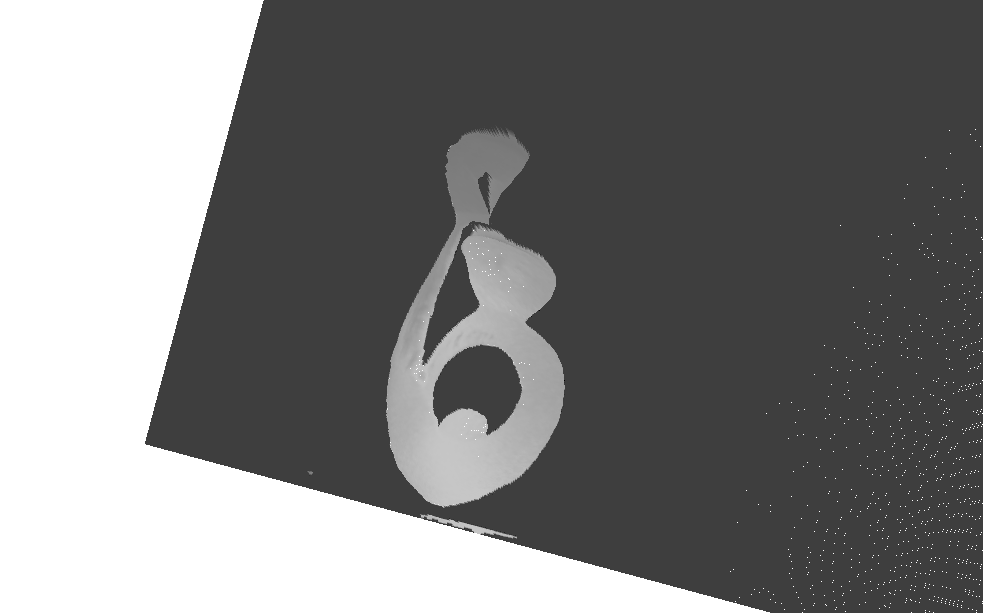
\includegraphics[width= 5cm]{3dniple02}
		\caption{Reconstrucción 3D de una figura abstracta ecuatoriana.}
		\label{niple}
\end{center}
\end{figure}

\section{Conclusión}
La reconstrucción de objetos en 3D, se hace todo en base a las probabilidades. Hemos notado que la gran mayoría de los métodos utilizados, lo que hacen es optimizar funciones que aproximan la representación del objeto en base a sus imágenes. Identificamos también que el procesamiento de previo que se le aplica a la imagen es de suma importancia, dado que nos permitirá obtener luego una mejor representación.

Luego de realizar una exhaustiva búsqueda de información y analizar los resultados de las reconstrucciones, hemos descubierto que es más complejo poder identificar los detalle de un objeto. También hemos podido observar que este campo ha ido en aumento ya sea por reconstrucciones en objetos en movimiento, de personas, de objetos con superficies no Lambertianas, mejoras de obtención de detalles, entre otros. Es necesario comprender cuales son las variables claves para la obtención de una reconstrucción de alta calidad, ya que la mayor complejidad se encuentra en calcular la estimación de la superficie o profundidad de un objeto.

Se puede apreciar el enfoque de Haque~\cite{ourpaper}, es mejorar la estimación de las profundidades utilizando un mapa de estas entregado por la Kinect y la ecuación de costos para calcularlo. Durante la investigación descubrimos que hay métodos mas robustos que la utilización de la relajación de Gauss-Seidel para las profundidad, algunos de estos son la utilización de Poisson, Multiple Process Unit (MPU), radial basis function (RBF), entre otros. Sin considerar que depende del enfoque que se le desee dar a la reconstrucción, es el método que se seleccionará para obtener la representación $3D$.

% references section

% can use a bibliography generated by BibTeX as a .bbl file
% BibTeX documentation can be easily obtained at:
% http://www.ctan.org/tex-archive/biblio/bibtex/contrib/doc/
% The IEEEtran BibTeX style support page is at:
% http://www.michaelshell.org/tex/ieeetran/bibtex/
\bibliographystyle{IEEEtran}
% argument is your BibTeX string definitions and bibliography database(s)
\bibliography{IEEEabrv,refs.bib}

% that's all folks

% don't panic!
\end{document}
